%%This is a very basic article template.
%%There is just one section and two subsections.
%--------------------------------------------------
\documentclass[letterpaper]{report}  
%--------------------------------------------------
%Packeges 
%--------------------------------------------------
\usepackage[english]{babel}
\usepackage{amsmath,amssymb,amsfonts} % Typical maths resource packages
\usepackage[dvips]{graphicx}
\usepackage{color}                    % For creating coloured text and background
\usepackage{fancyhdr}                 % For inclusion of title at the top of the page
\usepackage[left=3cm,right=1.5 cm,top=2cm,bottom=2cm,bindingoffset=0cm]{geometry}
\usepackage[explicit]{titlesec}
\usepackage{setspace}
\usepackage{pdfpages}
\usepackage{cite} 
\usepackage{float} 
\usepackage{newclude}
\usepackage{bookmark}
\usepackage{listings}
\usepackage{tikz}
\usepackage{type1cm}
\usepackage{textcomp}
\usepackage{hyperref}                  % For creating hyperlinks in cross
\usetikzlibrary{fit}
   
\definecolor{mygreen}{RGB}{28,172,0} % color values Red, Green, Blue
\definecolor{mylilas}{RGB}{170,55,241}
\definecolor{grey}{rgb}{0.97,0.97,0.97}
\newcommand*\chapterlabel{}
\makeatletter
\def\@makechapterhead#1{%
  \vspace*{10\p@}%
  {\parindent \z@ \centering \reset@font
        \par\nobreak
        \vspace*{2\p@}%
        {\Huge \bfseries \thechapter\quad #1\par\nobreak}
        \par\nobreak
        \vspace*{2\p@}%
    \vskip 40\p@
    %\vskip 100\p@
  }}
\def\@makeschapterhead#1{%
  \vspace*{10\p@}%
  {\parindent \z@ \centering \reset@font
        \par\nobreak
        \vspace*{2\p@}%
        {\Huge \bfseries #1\par\nobreak}
        \par\nobreak
        \vspace*{2\p@}%
    \vskip 100\p@
    %\vskip 100\p@
  }}
\makeatother

\newcounter{N}
\setlength{\parindent}{0ex}
\setlength{\parskip}{1em}

\lstset{language=Matlab,
basicstyle=\footnotesize\ttfamily,
basewidth=0.5em,
morekeywords={matlab2tikz},
keywordstyle=\color{blue},%
morekeywords=[2]{1}, keywordstyle=[2]{\color{black}},
identifierstyle=\color{black},%
stringstyle=\color{mylilas},
commentstyle=\color{mygreen},%
numbers=none,
numberstyle=\tiny\color{black},
stepnumber=2, 
numbersep=10pt,
tabsize=4,
aboveskip=3mm,
belowskip=3mm,
backgroundcolor=\color{grey},
frame=none,
showspaces=false,
showstringspaces=false,
breaklines=true}

\begin{document}
\begin{titlepage}
\begin{center}
\vspace{5cm}
{\bfseries\href{https://www.portfolioeffect.com}{www.portfolioeffect.com} \\
High Frequency Portfolio Analytics\\}
\vspace{8cm}
{\huge User Manual \\}
\vspace{0.3cm}
{\Huge\bfseries PortfolioEffectHFT \\ MATLAB Toolbox \\}
\vspace{0.4cm}
{\Large High Frequency Portfolio Backtesting \& Optimization \\}
% ----------------------------------------------------------------
\vspace{1.5cm}
{Andrey Kostin \\ andrey.kostin@portfolioeffect.com} \\[14pt]
 % ----------------------------------------------------------------
\vfill
\emph{{Released Under BSD License\\ by Snowfall Systems,
Inc.}}\\[2cm]
{August 20, 2015}
\end{center}
\end{titlepage}

\bookmarksetup{startatroot}
\cleardoublepage
\phantomsection
\addcontentsline{toc}{chapter}{Contents}
\bibliographystyle{amsplain}%}
\renewcommand{\bibname}{Contents}
\tableofcontents 

\chapter{Toolbox Installation}
PortfolioEffectHFT toolbox for MATLAB is provided as a zip archive for all
types of operating systems and as a self-install executable file for Windows. 

\section{Zip Archive (All OS)}
Download zip archive with a toolbox from PortfolioEffect  
\href{https://www.portfolioeffect.com/docs/platform/quant/tools/matlab}{downloads}
section or MATLAB Central 
\href{http://www.mathworks.com/matlabcentral/fileexchange/53194-portfolioeffecthft-high-frequency-trading-toolbox}{File Exchange}.

Once downloaded, unpack archive into the folder and add the 
PortfolioEffectHFT folder to MATLAB's path using ``Set Path'' menu. 
Then call any method of the package in
MATLAB editor to continue with the set-up:
\begin{lstlisting}
+++++++++++++++++++++++++++++++++++++++++++++++++
Welcome to PortfolioEffectHFT Toolbox.

Setup will download required binary files (~5mb).
Please, wait...
SUCCESS. File downloaded to: 
/home/appadmin/.matlab/R2015a/portfolioeffect-quant-client-1.0-allinone.jar
Updating java class path file...
SUCCESS. Java class path updated.

Setup complete! Restart Matlab session now.
+++++++++++++++++++++++++++++++++++++++++++++++++
\end{lstlisting}

Restart MATLAB to complete installation.

\section{Install Wizard (Windows)}
Download self-install executable for Windows from PortfolioEffect 
\href{https://www.portfolioeffect.com/docs/platform/quant/tools/matlab}{downloads}
section.
Follow the installation instructions. Once the wizard completes, add the 
PortfolioEffectHFT folder to MATLAB's path using ``Set Path''
menu.
The PortfolioEffectHFT toolbox is now fully configured. 

\chapter{Account Credentials}
All portfolio computations are performed on PortfolioEffect cloud servers.
To obtain a free non-professional account, you need to follow a quick sign-up
process on our website:
\href{https://www.portfolioeffect.com/registration}{www.portfolioeffect.com/registration}.\par
Please use a valid sign-up address - it will be used to email your
account activation link.

\section{Locate API Credentials} 
Log in to you account and locate your API credentials on the main page

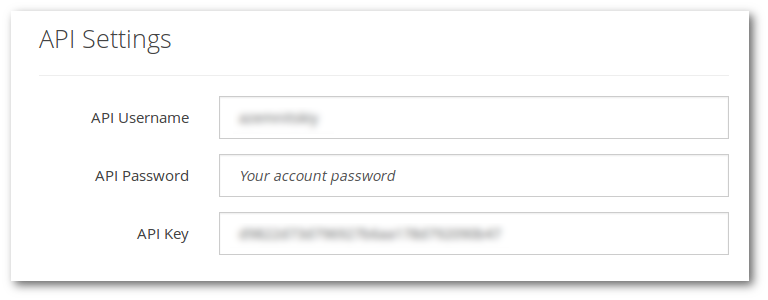
\includegraphics[width=5in,natwidth=768,natheight=300]{img/api-settings.png}
 
\section{Set API Credentials in MATLAB} 
Run the following commands to set your account API credentials for the
PortfolioEffectHFT Toolbox for MATLAB.
You will need to do it only once as your credentials are stored between sessions
on your local machine to speed up future logons. \par You would need to repeat
this procedure if you change your account password or install PortfolioEffect
HFT toolbox on another computer.
\begin{lstlisting}
util_setCredentials('API Username', 'API Password', 'API Key');
\end{lstlisting}
You are now ready to call PortfolioEffect methods.


\chapter{Portfolio Construction}
\section{User Data}
Users may supply their own historical datasets for index and position entries. 
This external data could be one a OHLC bar column element (e.g. 1-second close prices) or a vector of actual transaction prices that contains non-equidistant data points. 
You might want to prepend at least N =(4 x windowLength) data points to the
beginning of the interval of interest which would be used for initial calibration of portfolio metrics.
\subsection{Create Portfolio} 
Method
\href{https://www.portfolioeffect.com/docs/platform/quant/functions/general-functions/portfolio-create}{portfolio\_create()}.
takes a vector of index prices in the format (UTC timestamp, price) with UTC
timestamp expressed in milliseconds from 1970-01-01 00:00:00 EST.
\begin{lstlisting}
      Time          Value
 [1,] 1412256601000 99.30
 [2,] 1412256602000 99.33
 [3,] 1412256603000 99.30
 [4,] 1412256604000 99.26
 [5,] 1412256605000 99.36
 [6,] 1412256606000 99.36
 [7,] 1412256607000 99.36
 [8,] 1412256608000 99.38
 [9,] 1412256609000 99.40
[10,] 1412256610000 99.37
\end{lstlisting}
If index symbol is specified, it is silently ignored.
\begin{lstlisting}
data_spy=importdata('data_spy.mat'); 

% Create portfolio
portfolio=portfolio_create('priceDataIx',data_spy);
\end{lstlisting}

\subsection {Add Positions}
Positions are added using 
\href{https://www.portfolioeffect.com/docs/platform/quant/functions/general-functions/portfolio-add-position}{portfolio\_addPosition()}
with 'priceData' in the same format as index price.
\begin{lstlisting}
data_goog=importdata('data_goog.mat');
data_aapl=importdata('data_aapl.mat');

% Single position without rebalancing
portfolio_addPosition(portfolio,'GOOG',100,'priceData',data_goog); 

% Single position with rebalancing
portfolio_addPosition(portfolio,'AAPL',[300,150],'time',[1412266600000,1412276600000],'priceData',data_aapl); 
\end{lstlisting}

\section{Server Data}
At PortfolioEffect we are capturing and storing 1-second intraday bar history for a 
\href{https://www.portfolioeffect.com/docs/symbology}{all NASDAQ traded equites}.
This server-side dataset spans from January 2013 to the latest trading time minus five minutes. 
It could be used to construct asset portfolios and compute intraday portfolio metrics.
\subsection {Create Portfolio}
Method
\href{https://www.portfolioeffect.com/docs/platform/quant/functions/general-functions/portfolio-create}{portfolio\_create()}
creates new asset portfolio or overwrites an existing portfolio object with the
same name. \par
When using server-side data, it only requires a time interval that would be
treated as a default position holding period unless positions are added with rebalancing.
Index symbol could be specified as well with a default value of ``SPY'' - SPDR
S\&P 500 ETF Trust.
\par
Interval boundaries are passed in the following format:
\begin{itemize} 
  \item ``yyyy-MM-dd HH:MM:SS'' (e.g. ``2014-10-01 09:30:00'')
  \item ``yyyy-MM-dd'' (e.g. ``2014-10-01'')
  \item ``t-N'' (e.g. ``t-5'' is latest trading time minus 5 days)
  \item UTC timestamp in milliseconds (mills from ``1970-01-01 00:00:00'') in EST
  time zone
\end{itemize}
\begin{lstlisting}
% Timestamp in "yyyy-MM-dd HH:MM:SS" format
portfolio=portfolio_create('fromTime','2014-10-01 09:30:00','toTime','2014-10-02 16:00:00');

% Timestamp in "yyyy-MM-dd" format
portfolio=portfolio_create('fromTime','2014-10-01','toTime','2014-10-02');


% Timestamp in "t-N" format
portfolio=portfolio_create('fromTime','t-5','toTime','t');
\end{lstlisting}

\subsection {Add Positions}
Positions are added by calling
\href{https://www.portfolioeffect.com/docs/platform/quant/functions/general-functions/portfolio-add-position}{portfolio\_addPosition()}
method on a portfolio object with a list of symbols and quantities. For
positions that were rebalanced or had non-default holding periods a 'time' argument could be used to specify rebalancing timestamps.
\begin{lstlisting}
% Single position without rebalancing
portfolio_addPosition(portfolio,'GOOG',200);


% Multiple positions without rebalancing
portfolio_addPosition(portfolio,{'C','GOOG'},[300,200]);

% Single position with rebalancing
portfolio_addPosition(portfolio,'AAPL',[300,150],'time',['2014-10-02 09:30:01';'2014-10-02 11:30:01']);
\end{lstlisting}


\chapter{Portfolio Settings}
\section{Portfolio Metrics}
These settings regulate how portfolio returns and return moments are computed
\subsection {Portfolio Metrics Mode}
One of the two modes for collecting portfolio metrics that could be used:
\begin{itemize} 					
	\item ``portfolio''- portfolio metrics are computed using previous history of position rebalancing.
						 Portfolio risk and performance metrics account for the periods with no
						 market exposure (i.e. when no positions are held) depending on the
						 holding periods accounting settings (see holding periods mode below).
	\item ``price'' -    at any given point of time, both position and portfolio
						 metrics are computed for a buy-and-hold strategy. 
						 This mode is a common for classic portfolio theory and is often used in
						 academic literature for portfolio optimization or when computing price
						 statistics.
\end{itemize}
By default, mode is set to "portfolio".
\begin{lstlisting}
portfolio=portfolio_create('fromTime','2014-10-01 09:30:00','toTime','2014-10-02 16:00:00');
						   
portfolio_addPosition(portfolio,{'C','GOOG'},[300,200]);

% "price" mode
portfolio_settings(portfolio,'portfolioMetricsMode','price')
variance_price=portfolio_variance(portfolio);

% "portfolio" mode
portfolio_settings(portfolio,'portfolioMetricsMode','portfolio')
variance_portfolio=portfolio_variance(portfolio);

util_plot2d(variance_price,'price', 'title','Variance, portfolioMetricsMode')+...
util_line2d(variance_portfolio, 'portfolio')
\end{lstlisting}

\subsection {Holding Periods Only}
This setting should only be used when portfolio metrics mode is set to "portfolio".
When holdingPeriodsOnly is set to FALSE, trading strategy risk and performance
metrics will be annualized to include time intervals when strategy had no market exposure at certain points (i.e. when position quantity were zero).
When set to TRUE, trading strategy metrics are annualized only based on actual holding intervals.

\begin{lstlisting}
portfolio=portfolio_create('fromTime','2014-10-01 09:30:00','toTime','2014-10-02 16:00:00');

portfolio_addPosition(portfolio,'AAPL',[300,0,150],'time',['2014-10-01 09:30:00';'2014-10-01 13:30:00';'2014-10-02 13:30:00']);

% enable holdingPeriodsOnly
portfolio_settings(portfolio, 'holdingPeriodsOnly','true');
variance_holdingPeriodsOnly_TRUE=portfolio_variance(portfolio);

% disable holdingPeriodsOnly
portfolio_settings(portfolio, 'holdingPeriodsOnly','false');
variance_holdingPeriodsOnly_FALSE=portfolio_variance(portfolio);

util_plot2d(variance_holdingPeriodsOnly_TRUE,'true', 'title','Variance,holdingPeriodsOnly')+...
util_line2d(variance_holdingPeriodsOnly_FALSE, 'false')
\end{lstlisting}

\begin{lstlisting}
portfolio=portfolio_create('fromTime','2014-10-01 09:30:00','toTime','2014-10-02 16:00:00');

portfolio_addPosition(portfolio,{'C','GOOG'},[-300,200]);

% weights are normalized based on a simple sum (Markowitz)
portfolio_settings(portfolio, 'shortSalesMode','markowitz');
variance_markowitz=portfolio_variance(portfolio);

% weights are normalized based on a sum of absolute values (Lintner)
portfolio_settings(portfolio, 'shortSalesMode','lintner');
variance_lintner=portfolio_variance(portfolio);

util_plot2d(variance_markowitz,'markowitz', 'title','Variance,shortSalesMode')+...
util_line2d(variance_lintner, 'lintner')
\end{lstlisting}

\subsection {Short Sales Mode}
This setting is used to specify how position weights are computed. Available modes are:
\begin{itemize} 
  \item  ``lintner'' - the sum of absolute weights is equal to 1 (Lintner
  assumption)
  \item ``markowitz'' - the sum of weights must equal to 1 (Markowitz
  assumption)
\end{itemize}
Defaults to "lintner", which implies that the sum of absolute weights is used to normalize investment weights.

\section{Data Sampling}
These settings regulate how results of portfolio computations are returned. 
Depending on your usage scenario, some of them might bring significantly improvement to speed of your portfolio computations
\subsection{Results Sampling Interval}
Interval to be used for sampling computed results before returning them to the caller. 
Available interval values are: 
\begin{itemize} 
  \item ``Xs'' - seconds
  \item ``Xm'' - minutes
  \item ``Xh'' - hours
  \item ``Xd'' - trading days (6.5 hours in a trading day)
  \item ``Xw'' - weeks (5 trading days in 1 week)
  \item ``Xmo'' - month (21 trading day in 1 month)
  \item ``Xy'' - years (256 trading days in 1 year)
  \item ``none'' - no sampling.
  \item ``last'' - only the very last data point is returned  
\end{itemize}
Large sampling interval would produce smaller vector of results and would require less time spent on data transfer. 
Default value of ``1s'' indicates that data is returned for every second during
trading hours.
\begin{lstlisting}
portfolio=portfolio_create('fromTime','2014-10-01 09:30:00','toTime','2014-10-01 16:00:00');

portfolio_addPosition(portfolio,{'C','GOOG'},[300,200]);

% sample results every 30 seconds
portfolio_settings(portfolio, 'resultsSamplingInterval','30s');
variance_30s=portfolio_variance(portfolio);

% sample results every 5 minutes
portfolio_settings(portfolio, 'resultsSamplingInterval','15m');
variance_15m=portfolio_variance(portfolio);

util_plot2d(variance_30s,'30s', 'title','Variance,resultsSamplingInterval')+...
util_line2d(variance_15m, '15m')
\end{lstlisting}
\subsection{Input Sampling Interval}
Interval to be used as a minimum step for sampling input prices. Available interval values are: 
\begin{itemize} 
  \item ``Xs'' - seconds
  \item ``Xm'' - minutes
  \item ``Xh'' - hours
  \item ``Xd'' - trading days (6.5 hours in a trading day)
  \item ``Xw'' - weeks (5 trading days in 1 week)
  \item ``Xmo'' - month (21 trading day in 1 month)
  \item ``Xy'' - years (256 trading days in 1 year)
  \item ``none'' - no sampling
\end{itemize}
Default value is ``none'', which indicates that no sampling is applied.
\begin{lstlisting}
portfolio=portfolio_create('fromTime','2014-10-01 09:30:00','toTime','2014-10-02 16:00:00');

portfolio_addPosition(portfolio,{'C','GOOG'},[300,200]);

% sample input prices every 30 seconds
portfolio_settings(portfolio, 'inputSamplingInterval','30s');
variance_30s=portfolio_variance(portfolio);

% sample input prices every 5 min
portfolio_settings(portfolio, 'inputSamplingInterval','5m');
variance_5m=portfolio_variance(portfolio);

util_plot2d(variance_30s,'30s', 'title','Variance,inputSamplingInterval')+...
util_line2d(variance_5m, '5m')
\end{lstlisting}


\section{Model Pipeline}
\subsection{Window Length}
Specifies rolling window length that should be used for computing portfolio and position metrics. 
When portfolio mode is set to ``portfolio'', it is also the length of rebalancing history window to be used.
Available interval values are:
\begin{itemize} 
  \item ``Xs'' - seconds
  \item ``Xm'' - minutes
  \item ``Xh'' - hours
  \item ``Xd'' - trading days (6.5 calendar hours in a trading day)
  \item ``Xw'' - weeks (5 trading days in 1 week)
  \item ``Xmo'' - month (21 trading day in 1 month)
  \item ``Xy'' - years (256 trading days in 1 year)
  \item ``all'' - all observations are used
\end{itemize}
Default value is ``1d'' - one trading day.
\begin{lstlisting}
portfolio=portfolio_create('fromTime','2014-10-01 09:30:00','toTime','2014-10-02 16:00:00');

portfolio_addPosition(portfolio,{'C','GOOG'},[300,200]);

% 1 hour rolling window
portfolio_settings(portfolio, 'windowLength','1h');
variance_1h=portfolio_variance(portfolio);

% 1 week rolling window
portfolio_settings(portfolio, 'windowLength','1d');
variance_1d=portfolio_variance(portfolio);

util_plot2d(variance_1h,'1h', 'title','Variance,windowLength')+...
util_line2d(variance_1d, '1d')
\end{lstlisting}

\subsection{Time Scale}
Interval to be used for scaling return distribution statistics and producing metrics forecasts at different horizons. Available interval values are: 
\begin{itemize} 
  \item ``Xs'' - seconds
  \item ``Xm'' - minutes
  \item ``Xh'' - hours
  \item ``Xd'' - trading days (6.5 hours in a trading day)
  \item ``Xw'' - weeks (5 trading days in 1 week)
  \item ``Xmo'' - month (21 trading day in 1 month)
  \item ``Xy'' - years (256 trading days in 1 year)
  \item ``all'' - actual interval specified during portfolio creation.
\end{itemize}
Default value is "1d" - one trading day.
\begin{lstlisting}
portfolio=portfolio_create('fromTime','2014-10-01 09:30:00','toTime','2014-10-02 16:00:00');

portfolio_addPosition(portfolio,{'C','GOOG'},[300,200]);

% 1 hour time scale 
portfolio_settings(portfolio, 'timeScale','1h');
variance_1h=portfolio_variance(portfolio);

% 1 week time scale
portfolio_settings(portfolio, 'timeScale','1d');
variance_1d=portfolio_variance(portfolio);

util_plot2d(variance_1h,'1h', 'title','Variance,timeScale')+...
util_line2d(variance_1d, '1d')
\end{lstlisting}

\subsection{Microstructure Noise Model}
Enables market microstructure noise model of distribution returns.\\
Defaults to TRUE, which means that microstructure effects are modeled and resulting HF noise is removed from metric calculations. 
When FALSE, HF microstructure noise is not separated from asset returns, which at high trading frequencies could yield noise-contaminated results.

\begin{lstlisting}
portfolio=portfolio_create('fromTime','2014-10-01 09:30:00','toTime','2014-10-02 16:00:00');

portfolio_addPosition(portfolio,{'C','GOOG'},[300,200]);

% HF noise model is enabled
portfolio_settings(portfolio, 'noiseModel','true');
variance_noiseModel_TRUE=portfolio_variance(portfolio);

% HF noise model is disabled
portfolio_settings(portfolio, 'noiseModel','false');
variance_noiseModel_FALSE=portfolio_variance(portfolio);

util_plot2d(variance_noiseModel_TRUE,'true', 'title','Variance,noiseModel')+...
util_line2d(variance_noiseModel_FALSE, 'false')
\end{lstlisting}

\subsection{Jumps/Outliers Model}
Used to select jump filtering mode when computing return statistics. Available modes are: 
\begin{itemize} 
  \item ``none'' - price jumps are not filtered anywhere
  \item ``moments'' - price jumps are filtered only when computing return moments
  (i.e. for expected return, variance, skewness, kurtosis and derived
  metrics)
  \item ``all'' - price jumps are filtered from computed returns, prices and all
   return metrics.
\end{itemize}
\begin{lstlisting}
portfolio=portfolio_create('fromTime','2014-10-01 09:30:00','toTime','2014-10-04 16:00:00');

portfolio_addPosition(portfolio,{'C','GOOG'},[300,200]);

% Price jumps detection is enabled for returns and moments
portfolio_settings(portfolio, 'jumpsModel','all');
variance_all=portfolio_variance(portfolio);

% Price jumps detection is disabled
portfolio_settings(portfolio, 'jumpsModel','none');
variance_none=portfolio_variance(portfolio);

util_plot2d(variance_all,'all', 'title','Variance,jumpsModel')+...
util_line2d(variance_none, 'none')
\end{lstlisting}

\subsection {Density Model}
Used to select density approximation model of return distribution. Available models are:
\begin{itemize} 
  \item ``GLD'' - Generalized Lambda Distribution
  \item ``CORNER\_FISHER'' - Corner-Fisher approximation
  \item ``NORMAL'' - Gaussian distribution
\end{itemize}
Defaults to ``GLD'', which would fit a very broad range of distribution shapes.

\begin{lstlisting}
portfolio=portfolio_create('fromTime','2014-10-01 09:30:00','toTime','2014-10-02 16:00:00');

portfolio_addPosition(portfolio,{'C','GOOG'},[300,200]);

% Using normal density
portfolio_settings(portfolio, 'densityModel','NORMAL');
util_plotDensity(portfolio_pdf(portfolio,0.6,1,100,true))

% Using Generalized Lambda density
portfolio_settings(portfolio, 'densityModel','GLD');
util_plotDensity(portfolio_pdf(portfolio,0.6,1,100,true))
\end{lstlisting}

\subsection {Factor Model}
Factor model to be used when computing portfolio metrics. Available models are: 
\begin{itemize} 
  \item ``sim'' - portfolio metrics are computed using the Single Index Model
  \item ``direct'' - portfolio metrics are computed using portfolio value itself
  (experimental)
\end{itemize}
Defaults to "sim", which implies that the Single Index Model is used to compute portfolio metrics.

\begin{lstlisting}
portfolio=portfolio_create('fromTime','2014-10-01 09:30:00','toTime','2014-10-02 16:00:00');

portfolio_addPosition(portfolio,{'C','GOOG'},[300,200]);

% Single Index Model is used
portfolio_settings(portfolio, 'factorModel','sim');
variance_sim=portfolio_variance(portfolio);

% Direct model is used
portfolio_settings(portfolio, 'factorModel','direct');
variance_direct=portfolio_variance(portfolio);

util_plot2d(variance_sim,'sim', 'title','Variance,factorModel')+...
util_line2d(variance_direct, 'direct')
\end{lstlisting}

\subsection{Drift Term}
Used to enable drift term (expected return) when computing probability density approximation and related metrics (e.g. CVaR, Omega Ratio, etc.).
Defaults to TRUE, which implies that distribution is centered around expected return.

\begin{lstlisting}
portfolio=portfolio_create('fromTime','2014-10-01 09:30:00','toTime','2014-10-02 16:00:00');

portfolio_addPosition(portfolio,{'C','GOOG'},[300,200]);

% Drift term is enabled
portfolio_settings(portfolio, 'driftTerm','true');
CVaR_driftTerm_TRUE=portfolio_CVaR(portfolio,0.05);

% Drift term is disabled
portfolio_settings(portfolio, 'driftTerm','false');
CVaR_driftTerm_FALSE=portfolio_CVaR(portfolio,0.05);

util_plot2d(CVaR_driftTerm_TRUE,'sim', 'title','CVaR,driftTerm')+...
util_line2d(CVaR_driftTerm_FALSE, 'direct')
\end{lstlisting}

\section{Transactional Costs}
These settings provide a framework for adding variable and fixed transactional costs into return, expected return and profit calculations.
All metrics based on expected return like Sharpe Ratio, VaR (with drift term
enabled) would reflect transactional costs in their computations.
\subsection{Cost Per Share}
Amount of transaction costs per share. Default value is 0.
\begin{lstlisting}
portfolio=portfolio_create('fromTime','2014-10-01 09:30:00','toTime','2014-10-02 16:00:00');

portfolio_addPosition(portfolio,'AAPL',[300,100,50,150],'time',['2014-10-01 09:30:00';'2014-10-01 13:30:00';'2014-10-01 16:00:00';'2014-10-02 13:30:00']);

% Transactional costs per share are 0.5 cent 
portfolio_settings(portfolio, 'txnCostPerShare',0.05);
return_50=portfolio_return(portfolio);

% Transactional costs per share are 0.1 cent 
portfolio_settings(portfolio, 'txnCostPerShare',0.001);
return_1=portfolio_return(portfolio);

util_plot2d(return_50,'0.05', 'title','Return,txnCostPerShare')+...
util_line2d(return_1, '0.001')
\end{lstlisting}
\subsection {Cost Per Transaction}
Amount of fixed costs per transaction. Defaults to 0.
\begin{lstlisting}
portfolio=portfolio_create('fromTime','2014-10-01 09:30:00','toTime','2014-10-02 16:00:00');

portfolio_addPosition(portfolio,'AAPL',[300,100,50,150],'time',['2014-10-01 09:30:00';'2014-10-01 13:30:00';'2014-10-01 16:00:00';'2014-10-02 13:30:00']);

% Fixed costs per transaction are 9 dollars
portfolio_settings(portfolio, 'txnCostFixed',19);
return_19=portfolio_return(portfolio);

% Fixed costs per transaction are 1 dollar
portfolio_settings(portfolio, 'txnCostFixed',1);
return_1=portfolio_return(portfolio);

util_plot2d(return_19,'19', 'title','Return,txnCostFixed')+...
util_line2d(return_1, '1')
\end{lstlisting}

\chapter{Portfolio Optimization}

\section{Optimization Goals \& Constraints}
A classic problem of constructing a portfolio that meets certain maximization/minimization 
goals and constraints is addressed in our version of a multi-start portfolio optimization algorithm. At every time step
optimization algorithm tries to find position weights that best meet optimization goals and constraints.

\subsection{Key Features}
\begin{itemize} 
  \item A multi-start approach is used to compare local optima with each other and select a global optimum. 
		Local optima are computed using a modified method of parallel tangents (PARTAN).
  \item When optimization algorithm is supplied with mutually exclusive constraints, it would try to produce result that is equally close (in absolute terms) to all constraint boundaries. 
		For instance, constraints ``x > 6'' and ``x < 4'' are mutually exclusive, so
		the optimization algorithm would choose ``x = 5'', which is a value that has the smallest distance to both constraints.
  \item Portfolio metrics change over time, but optimization uses only the latest value in the time series.
		Therefore, the faster metric series would change, the more likely current optimal weights would deviate
		from the optimal weights at the next time step. 
  \item Optimization results depend on provided portfolio settings. 
		For example, short windowLength would produce "spot" versions of portfolio metrics and 
		computed optimal weights would change faster to reflect shortened metric horizon. 
\end{itemize}

\subsection{Optimization Goals}
Optimization algorithm requires a single maximization/minimization goal to be set using 
\href{https://www.portfolioeffect.com/docs/platform/quant/functions/optimization-functions/optimization-goal}{optimization\_goal()}
method that operates on a portfolio (see
\href{https://www.portfolioeffect.com/docs/platform/quant/manuals/portfolio-construction}{portfolio
construction}).
Returned optimizer object could be used to add optional optimization constraints and then passed to the 
\href{https://www.portfolioeffect.com/docs/platform/quant/functions/optimization-functions/optimization-run}{optimization\_run}
method to launch portfolio optimization.
\par

\begin{lstlisting}
portfolio=portfolio_create('fromTime','2014-10-01 09:30:00','toTime','2014-10-02 16:00:00');

portfolio_addPosition(portfolio,{'C','GOOG'},[300,200]);
portfolio_settings(portfolio,'portfolioMetricsMode','price','resultsSamplingInterval','30m');

% set optimization goal
optimizer=optimization_goal(portfolio,'goal','Return','direction','maximize');

% launch optimization and obtain optimal portfolio
optimalPortfolio=optimization_run(optimizer);

util_plot2d(portfolio_return(portfolio),'Simple Portfolio', 'title','Portfolio Return')+...
util_line2d(portfolio_return(optimalPortfolio), 'Optimal Portfolio')
\end{lstlisting}

The following portfolio metrics could currently be used as optimization goals:

\begin{description} 
\item[``Variance''] \hfill \\ 
portfolio returns variance 
\item[``VaR''] \hfill \\ 
portfolio Value-at-Risk
\item[``CVaR''] \hfill \\ 
portfolio Conditional Value-at-Risk (Expected Tail Loss)
\item[``ExpectedReturn''] \hfill \\ 
portfolio expected return
\item[``Return''] \hfill \\
portfolio return
\item[``SharpeRatio''] \hfill \\
portfolio Sharpe Ratio
\item[``ModifiedSharpeRatio''] \hfill \\
portfolio modified Sharpe Ratio
\item[``StarrRatio''] \hfill \\
portfolio STARR Ratio
\item[``ContraintsOnly''] \hfill \\
no optimization is performed. This is used for returning an arbitrary portfolio
that meets specified set of constraints
\item[``None''] \hfill \\  
no optimization is performed and constraints are not processes.
Portfolio positions are returned with equal weights
\end{description}

\subsection{Adding Constraints}
Optimization constraints cover both metric-based and weight-based
constraints. Metric-based constraints limit portfolio-level metrics to a certain
range of values. For example, zero beta constraint would produce market-neutral optimal portfolio.
Weight-based constraints operate on optimal position weights or sum of weights to 
give control over position concentration risks or short-sales assumptions.
\par
Constraint methods could be chained to produce complex optimization rules:
\par
Since position quantities are integer numbers and weights are decimals, a discretization error is introduced while converting optimal position weights to corresponding quantities. 
By default, optimal portfolio starts with a value of the initial portfolio. 
Portfolio value could be fixed to a constant level at every optimization step
(see corresponding constraint below).
Higher portfolio value could be used to keep difference between computed optimal weights and effective weights based on position quantities small.
Lower portfolio value or higher asset price would normally increase discretization error.

\begin{lstlisting}
% create portfolio and add positions
portfolio=portfolio_create('fromTime','2014-10-01 09:30:00','toTime','2014-10-02 16:00:00');

portfolio_addPosition(portfolio,{'C','GOOG'},[300,200]);
portfolio_settings(portfolio,'portfolioMetricsMode','price','resultsSamplingInterval','30m');

% set optimization goal
optimizer=optimization_goal(portfolio,'goal','SharpeRatio','direction','maximize');

% add constraints
optimization_constraint_beta(optimizer,'=',0);
optimization_constraint_weight(optimizer,'>=',0.5, 'C');
optimization_constraint_variance(optimizer,'<=',0.02);
 
% launch optimization and obtain optimal portfolio
optimalPortfolio=optimization_run(optimizer);

 util_plot2d(portfolio_sharpeRatio(portfolio),'Simple Portfolio', 'title','Sharpe Ratio')+...
util_line2d(portfolio_sharpeRatio(optimalPortfolio), 'Optimal Portfolio')

util_plot2d(portfolio_beta(portfolio),'Simple Portfolio', 'title','Beta')+...
util_line2d(portfolio_beta(optimalPortfolio), 'Optimal Portfolio')

util_plot2d(portfolio_variance(portfolio),'Simple Portfolio', 'title','Variance')+...
util_line2d(portfolio_variance(optimalPortfolio), 'Optimal Portfolio')
\end{lstlisting}

The following constraint methods are available:
			
\begin{description} 
\item[\href{https://www.portfolioeffect.com/docs/platform/quant/functions/optimization-functions/optimization-constraint-all-weights}{optimization\_constraint\_allWeights}]
\hfill \\
portfolio weights of all positions
\item[\href{https://www.portfolioeffect.com/docs/platform/quant/functions/optimization-functions/optimization-constraint-weight}{optimization\_constraint\_weight}]
\hfill \\
portfolio position weights
\item[\href{https://www.portfolioeffect.com/docs/platform/quant/functions/optimization-functions/optimization-constraint-sum-of-abs-weights}{optimization\_constraint\_sumOfAbsWeights}]
\hfill \\
portfolio's sum of absolute positions weights for selected positions
\item[\href{https://www.portfolioeffect.com/docs/docs/platform/quant/functions/optimization-functions/optimization-constraint-return}{optimization\_constraint\_return}]
\hfill \\
portfolio return
\item[\href{https://www.portfolioeffect.com/docs/platform/quant/functions/optimization-functions/optimization-constraint-expected-return}{optimization\_constraint\_expectedReturn}]
\hfill \\
portfolio expected return
\item[\href{https://www.portfolioeffect.com/docs/platform/quant/functions/optimization-functions/optimization-constraint-variance}{optimization\_constraint\_variance}]
\hfill \\
portfolio returns variance
\item[\href{https://www.portfolioeffect.com/docs/platform/quant/functions/optimization-functions/optimization-constraint-beta}{optimization\_constraint\_beta}]
\hfill \\
portfolio beta
\item[\href{https://www.portfolioeffect.com/docs/platform/quant/functions/optimization-functions/optimization-constraint-var}{optimization\_constraint\_VaR}]
\hfill \\
portfolio Value-at-Risk
\item[\href{https://www.portfolioeffect.com/docs/platform/quant/functions/optimization-functions/optimization-constraint-cvar}{optimization\_constraint\_CVaR}]
\hfill \\
portfolio Conditional Value-at-Risk (Expected Tail Loss)
\item[\href{https://www.portfolioeffect.com/docs/platform/quant/functions/optimization-functions/optimization-constraint-modified-sharpe-ratio}{optimization\_constraint\_modifiedSharpeRatio}]
\hfill \\
portfolio modified Sharpe Ratio
\item[\href{https://www.portfolioeffect.com/docs/platform/quant/functions/optimization-functions/optimization-constraint-sharpe-ratio}{optimization\_constraint\_sharpeRatio}]
\hfill \\
portfolio Sharpe Ratio
\item[\href{https://www.portfolioeffect.com/docs/platform/quant/functions/optimization-functions/optimization-constraint-starr-ratio}{optimization\_constraint\_starrRatio}]
\hfill \\
portfolio STARR Ratio
\end{description}

\subsection{Scalar Constraints}
Scalar constraints are the simplest type of optimization boundaries. 
They require a single constant that is applied over a full time span of portfolio optimization. 
An example below sets portfolio beta constraint to be greater or equal to 0.1.

\begin{lstlisting}
% create portfolio and add positions
portfolio=portfolio_create('fromTime','2014-10-01 09:30:00','toTime','2014-10-02 16:00:00');

portfolio_addPosition(portfolio,{'C','GOOG'},[300,200]);

% rebalancing every minute, static portfolio ignores rebalancing history
portfolio_settings(portfolio,'portfolioMetricsMode','price','resultsSamplingInterval','30m');

% set optimization goal and define constraints
optimizer=optimization_goal(portfolio,'goal','SharpeRatio','direction','maximize');
optimization_constraint_beta(optimizer, '<=',0.1);

% run optimization
optimalPortfolio=optimization_run(optimizer);

% plot results
util_plot2d(portfolio_beta(optimalPortfolio),'Optimal Beta', 'title','Beta')+...
util_line2d(portfolio_beta(portfolio), 'Original Beta')
\end{lstlisting}

\subsection{Vector Constraints}
Instead of using a single scalar, one could specify an vector of constraint values with corresponding timestamps. 
Optimization algorithm would then automatically determine when certain constraint value should be applied based on the current rebalancing time.

\begin{lstlisting}
% create portfolio and add positions
portfolio=portfolio_create('fromTime','2014-10-01 09:30:00','toTime','2014-10-02 16:00:00');

portfolio_addPosition(portfolio,{'AAPL','GOOG'},[500,600]);

% rebalancing every minute, static portfolio ignores rebalancing history
portfolio_settings(portfolio,'portfolioMetricsMode','price','resultsSamplingInterval','30m');

betaVector = [1412171500000,0.1; 1412262500000,0.5];

% set optimization goal and define constraints
optimizer=optimization_goal(portfolio,'goal','SharpeRatio','direction','maximize');
optimizer=optimization_constraint_beta(optimizer, '<=',betaVector);

% run optimization
optimalPortfolio=optimization_run(optimizer);

% plot results
util_plot2d(portfolio_beta(optimalPortfolio),'Optimal Beta', 'title','Beta')+...
util_line2d(portfolio_beta(portfolio), 'Original Beta')
\end{lstlisting}


%\subsection {User-Defined Constraints}
%User-defined constraint relies on a provided function, which is called during
% portfolio optimization at specified rebalancing times.
%Function should return a scalar constraint value and would optionally receive
% portfolio and current time, if they are specified as arguments.
%\begin{itemize} 
%  \item function () - automatically converted to a scalar constraint
%  \item function (time) - automatically converted to a vector constraint
%  \item function (portfolio, time) - evaluated during optimization procedure
%\end{itemize}
%
%\textbf{Note:} When functional constraint specifies portfolio object as a
% required argument, it could no longer be quickly converted to a scalar or vector-based constraint.
% In such case, optimization procedure would take a performance hit.
%
%\begin{lstlisting}
% create portfolio and add positions
% portfolio=portfolio_create('fromTime','2014-10-01
% 09:30:00','toTime','2014-10-02 16:00:00');
%
% portfolio_addPosition(portfolio,{'AAPL','GOOG'},[500,600]);
%
% rebalancing every 30m, static portfolio ignores rebalancing history
%portfolio_settings(portfolio,'portfolioMetricsMode','price','resultsSamplingInterval','30m');
%
% compute benchmark beta values
%bench_portfolio=portfolio_create('fromTime','2014-10-01
% 09:30:00','toTime','2014-10-02 16:00:00');
%
%portfolio_settings(bench_portfolio, 'resultsSamplingInterval','30m');
%portfolio_addPosition(bench_portfolio,'SPW', 1);
%bench_beta = portfolio_beta(bench_portfolio);
%
% define custom optimization constraint method for beta
%function [return] = myConstraint(portfolio, time)
% 
%  bench_beta_value = bench_beta(bench_beta(:,1)==time, 2);
%  portfolio_beta_value = portfolio_beta(portfolio)
%  portfolio_beta_value =
%  portfolio_beta_value(portfolio_beta_value(:,1)==time,2);
%  
%  if portfolio_beta_value > bench_beta_value 
%    return=bench_beta_value;
%  else  
%    return=portfolio_beta_value;
%  end
%  
%end
%
% set optimization goal and define constraints
%optimizer=optimization_goal(portfolio,'goal','SharpeRatio','direction','maximize');
% optimizer=optimization_constraint_beta(optimizer, '<=',myConstraint)
%
% run optimization
%optimalPortfolio=optimization_run(optimizer);
%
% plot results
%util_plot2d(portfolio_beta(optimalPortfolio),'Optimal Beta',
% 'title','Beta')+...
%util_line2d(portfolio_beta(portfolio), 'Original Beta')
%\end{lstlisting}

 
\end{document}
